% Provenance (never printed): old premiere S material on plate kinematics (rigid
% plates, rates from magnetic anomalies and from satellite positioning, hotspots
% and the Hawaiian chain, the coherence of the model); see
% sources/book2/PROVENANCE.md. Velocities from the NNR-MORVEL56 poles
% (figdata/grade-11/plate_velocities.py), station series from the Nevada Geodetic
% Laboratory (gnss_series.py), volcano ages from Clague and Dalrymple 1987
% (hawaii_chain.py). Euler poles and triple junctions belong to Year 1: the
% rotation pole is told, not defined.
\chapter{الصفائح وحركاتها}\label{ch:g11:plate-motions}

قرب قمة ماونا كيا، في جزيرة هاواي، يستقبل هوائي مثبت في
الصخر إشارات أقمار تحديد المواقع كل يوم منذ
أكتوبر 1996. وفي كل يوم يحسب حاسوب موقع الهوائي، بدقة بضعة
ملليمترات. وثلاثون سنة من المواقع تروي الحكاية نفسها كل سنة: فالهوائي
والجبل والجزيرة كلها تتحرك نحو \qty{7}{cm} في السنة
نحو الغرب الشمالي الغربي، دون توقف ودون انعطاف. وبحلول عام 2026 كان
الهوائي قد ابتعد أكثر من مترين عن موضعه الأول. يقيس هذا الفصل
حركات كهذه، ويبيّن كيف تتلاءم معًا على كرة، ويقرأ
الحركة نفسها في سلسلة البراكين الخامدة الممتدة من هاواي عبر
شمال المحيط الهادئ.
% ledger: data:b2-ngl-gnss

\begin{recall}
\omterm{def:g11:lithosphere-asthenosphere:lithosphere}{الغلاف الصخري} مقسم إلى صفائح تكتونية يتحرك بعضها بالنسبة إلى
بعض بضعة سنتيمترات في السنة؛ وحدودها ظهرات وخنادق
ونطاقات تصادم وصدوع تحويلية (الكتاب 1، الصف 7). والبقعة الساخنة موضع
عميق في الوشاح يغذي بركانًا على الصفيحة التي فوقه؛ فتحمل الصفيحة
البركان بعيدًا بينما ينمو بركان جديد فوق البقعة الساخنة (الكتاب 1،
الصف 7). ويحسب جهاز استقبال تحديد المواقع بالأقمار الصناعية موقعه انطلاقًا من
إشارات عدة أقمار (الكتاب 1، الصف 9). وتعطي الشرائط المغناطيسية
لقاع المحيط معدل توسع الظهرة
(\cref{ch:g11:drift-to-spreading})، \omterm{def:g11:lithosphere-asthenosphere:lithosphere}{والغلاف الصخري} هو الغلاف الخارجي
الصلب للأرض، وسمكه نحو \qty{100}{km}
(\cref{ch:g11:lithosphere-asthenosphere}). والسرعة \qty{1}{cm} في السنة تساوي
\qty{10}{km} في كل مليون سنة، و\qty{1}{mm} في السنة تساوي \qty{1}{km} في كل
مليون سنة.
\end{recall}

\begin{omfigure}
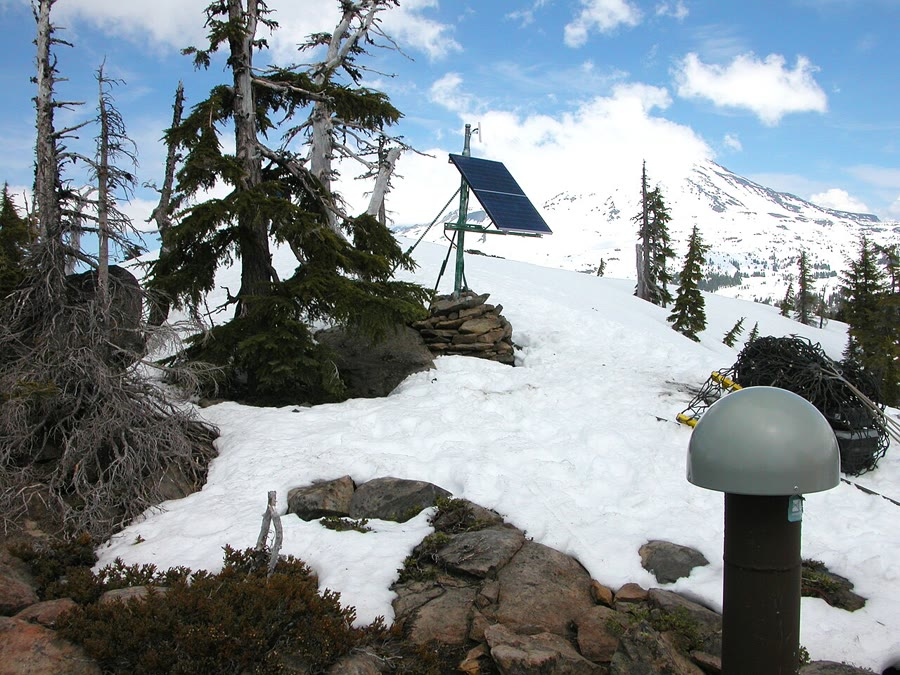
\includegraphics[width=0.62\linewidth]{images/book2/g11-usgs-gps-station.jpg}

{\small محطة دائمة لتحديد المواقع بالأقمار الصناعية على بركان في
سلسلة جبال كاسكيد، أوريغون (2007). يقع الهوائي تحت القبة الرمادية، على سارية
مثبتة بإحكام في الأرض؛ واللوح الشمسي خلفها يزود جهاز الاستقبال بالطاقة. ومحطة كهذه
تسجل موقعها يومًا بعد يوم. الصورة: ديف شيرود،
هيئة المسح الجيولوجي الأمريكية (ملك عام).}
\end{omfigure}
% ledger: photo:g11-gps-station

\section{صفائح صلبة على كرة}

الزلازل ليست مبعثرة عشوائيًا على الأرض: فكلها تقريبًا
تقع على امتداد أحزمة ضيقة، هي حدود الصفائح (الكتاب 1، الصف 7). أما داخل
الصفيحة فلا يكاد الصخر ينكسر. فالصفيحة إذن ليست جلدًا لينًا
يتمدد ويتجعد وهو يتحرك، بل قطعة صلبة من \omterm{def:g11:lithosphere-asthenosphere:lithosphere}{الغلاف الصخري}
تتحرك ككل.

\begin{definition}[الصفيحة الصلبة]\label{def:g11:plate-motions:rigid-plate}
\emph{الصفيحة الصلبة}\index{صفيحة صلبة} قطعة من \omterm{def:g11:lithosphere-asthenosphere:lithosphere}{الغلاف الصخري} تتحرك
ككتلة واحدة: فالمسافات بين نقاطها لا تتغير، وتشوهها
مجموع في نطاقات ضيقة على امتداد حدودها.
\end{definition}

نموذج الصفائح الصلبة تقريب. فبعض المناطق تتشوه على مئات
الكيلومترات، مثل الهضاب العالية خلف الهيمالايا أو غرب
أمريكا الشمالية، ويعاملها النموذج حدودًا عريضة. لكنه على معظم
سطح الأرض يعمل جيدًا على نحو لافت: فالسرعات التي يتنبأ بها
للصفائح الصلبة تطابق تلك التي تقيسها المحطات الساتلية في حدود بضعة
ملليمترات في السنة (\cref{sec:g11:plate-motions:predictive})، في حين تتحرك الصفائح
بعضها بالنسبة إلى بعض بالسنتيمترات في السنة.

كيف يمكن لقلنسوة صلبة أن تتحرك على سطح كرة؟ لا يمكنها أن تنزلق في
خط مستقيم، لأن الخط المستقيم يغادر الكرة. فأيًّا كانت حركة
القلنسوة الصلبة، فهي \emph{دوران} حول محور يمر بمركز
الأرض. ويلتقي المحور بالسطح عند \emph{قطب دوران} الصفيحة. والنقطة
على الصفيحة تتحرك على امتداد دائرة صغيرة حول ذلك القطب، وكلما
بعدت عن القطب كبرت دائرتها وازدادت سرعتها
(الشكل أدناه). أما البرهان على أن كل حركة
لقلنسوة صلبة دوران كهذا، واستعمال أقطاب الدوران لوصف حدود
الصفائح، فموضعهما الكتاب~3؛ ولا تُستعمل هنا إلا السرعات.

\begin{omfigure}
\begin{tikzpicture}[scale=1.15, font=\footnotesize]
  \fill[omSea!45] (0,0) circle (2);
  \draw (0,0) circle (2);
  % small circles about the rotation pole (pole at the top), seen slightly from above
  \foreach \a/\len in {60/0.75, 35/1.23, 0/1.5} {
    \pgfmathsetmacro{\r}{2*cos(\a)}
    \pgfmathsetmacro{\h}{2*sin(\a)}
    \draw[black!45, densely dashed] (-\r,\h) arc[start angle=180, end angle=0, x radius=\r, y radius=0.22*\r];
    \draw[omDef!80!black, line width=0.7pt] (-\r,\h) arc[start angle=180, end angle=360, x radius=\r, y radius=0.22*\r];
    \draw[-{Stealth[length=5pt]}, omProp, line width=1.1pt] (0,\h-0.22*\r) -- ++(\len,0);
  }
  \draw[black!70, dash pattern=on 3pt off 2pt] (0,-2.5) -- (0,2.55);
  \fill (0,2) circle (1.6pt);
  \node[anchor=south west] at (0.05,2.02) {قطب الدوران};
  \node[anchor=north, text=black!70] at (0,-2.5) {محور الدوران، يمر بالمركز};
  \fill (0,0) circle (1pt);
  \node[anchor=west, align=left] at (2.25,0.9) {كل نقطة تتحرك\\على امتداد دائرة صغيرة\\حول القطب};
  \node[anchor=west, align=left, text=omProp] at (2.25,-0.4) {السرعة: أكبر ما تكون\\\foreignlanguage{arabic}{على بعد \babelsublr{\ang{90}} من القطب}};
\end{tikzpicture}

{\small تدور \omterm{def:g11:plate-motions:rigid-plate}{صفيحة صلبة} على كرة حول محور يمر بمركز
الأرض. فالنقاط القريبة من قطب الدوران تتحرك ببطء، على امتداد دوائر صغيرة؛ أما
النقاط الواقعة على بعد \ang{90} من القطب فهي الأسرع (الأسهم: سرعات بمقياس رسم حقيقي).}
\end{omfigure}

من السهل حساب سرعة نقطة. فالنقطة الواقعة على بعد زاوي
$\theta$ من القطب تقع على المسافة $R\sin\theta$ من المحور، حيث
$R = \qty{6371}{km}$ نصف قطر الأرض. فإذا دارت الصفيحة بمقدار $\omega$
درجة في كل مليون سنة، قطعت النقطة الكسر $\omega/360$ من
الدائرة التي نصف قطرها $R\sin\theta$ في مليون سنة:
\[
  v = \frac{\omega}{360} \times 2\pi R\sin\theta
    = \frac{\pi\,\omega}{180}\,R\sin\theta .
\]
ومن أجل $\omega = \qty{1}{\degree}$ في كل مليون سنة و$\theta = \ang{90}$
يكون هذا $\pi \times 6371/180 \approx \qty{111}{km}$ في كل مليون سنة، أي
\qty{11.1}{cm} في السنة. فليس للصفيحة إذن سرعة واحدة: فنقاطها تتحرك
بسرعات تتراوح بين الصفر عند قطب الدوران (إن وقع القطب على
الصفيحة) وقيمة عظمى على بعد \ang{90} منه. والصدوع التحويلية على امتداد الظهرة،
التي تسمح لصفيحتين بالانزلاق إحداهما بمحاذاة الأخرى، تمتد على دوائر صغيرة حول
قطب الدوران النسبي للصفيحتين.
% ledger: earth:Rmean (shared), nnr56:poles

تعطي المجموعات المنشورة لأقطاب الدوران، لكل صفيحة، موقع
قطبها ومعدل دورانها. وإحداها، المبنية أساسًا من معدلات
التوسع واتجاهاته المقيسة على امتداد الظهرات، تصف 56
صفيحة؛ فالصفيحة الهادئية تدور بمقدار
\ang{0.651} في كل مليون سنة، والصفيحة الأوراسية بمقدار \ang{0.223}. ومن هذه
الأرقام يحسب الحاسوب سرعة أي نقطة من أي صفيحة
(الخريطة أدناه).
% ledger: nnr56:poles, nnr56:data

\begin{omfigure}
\begin{tikzpicture}
\begin{axis}[ommap, width=\linewidth, xtick={-180,-90,...,180}, ytick={-60,0,60}]
\addplot[fill=omLithAlluv, draw=black!45, line width=0.2pt] table {figdata/out/shared-geo-land.dat};
\addplot[omRidge, line width=0.6pt] table {figdata/out/shared-geo-school-ridge.dat};
\addplot[omRidge!70!black, line width=0.6pt] table {figdata/out/shared-geo-school-transform.dat};
\addplot[omTrench, line width=0.6pt] table {figdata/out/shared-geo-school-subduction.dat};
\addplot[fill=omTrench, draw=none] table {figdata/out/shared-geo-school-teeth.dat};
\addplot[black!65, line width=0.6pt] table {figdata/out/shared-geo-school-collision.dat};
% computed in figdata/grade-11/plate_velocities.py (NNR-MORVEL56); 2.5 degrees per cm/yr
\addplot[black, line width=0.8pt, -{Stealth[length=4pt]}, quiver={u=\thisrow{dx}, v=\thisrow{dy}}]
  table[x=lon, y=lat] {figdata/out/grade-11-plate_velocities-arrows.dat};
\addplot[omProp, line width=1.2pt, -{Stealth[length=5pt]}, quiver={u=\thisrow{dx}, v=\thisrow{dy}}]
  table[x=lon, y=lat] {figdata/out/grade-11-plate_velocities-hawaii.dat};
\addplot[only marks, mark=*, mark size=1.3pt, omProp] coordinates {(-155.46,19.80)};
\node[font=\scriptsize, anchor=north, fill=white, fill opacity=0.75, text opacity=1, inner sep=1pt]
  at (axis cs:-150,15) {ماونا كيا};
\draw[black, line width=0.8pt, -{Stealth[length=4pt]}] (axis cs:-172,-80) -- (axis cs:-147,-80);
\node[font=\scriptsize, anchor=west, fill=white, fill opacity=0.75, text opacity=1, inner sep=1pt]
  at (axis cs:-145,-80) {\foreignlanguage{arabic}{\babelsublr{\qty{10}{cm}} في السنة}};
\end{axis}
\end{tikzpicture}

{\small سرعات نقاط داخل 16 صفيحة، محسوبة من أقطاب
دورانها المنشورة، في إطار لا يدور فيه \omterm{def:g11:lithosphere-asthenosphere:lithosphere}{الغلاف الصخري} ككل.
وتتحرك الصفائح الهادئية ونازكا وكوكوس والأسترالية والهندية أسرع ما يكون؛
والصفائح الأوراسية وأمريكا الشمالية وأمريكا الجنوبية والقطبية الجنوبية ببطء. السهم الأحمر:
الصفيحة الهادئية عند ماونا كيا. أقطاب الدوران: أرغوس وغوردون وديميتس
(2011)؛ حدود الصفائح: بيرد (2003)؛ اليابسة: Natural Earth.}
\end{omfigure}
% ledger: nnr56:poles, data:pb2002, data:ne-land

\section{قياس الحركات}

\subsection{طريقتان لقياس السرعة}

تعطي الشرائط المغناطيسية لقاع المحيط السرعة التي تتباعد بها صفيحتان
عبر ظهرة (\cref{ch:g11:drift-to-spreading}): اقسم
بعد الشريط عن محور الظهرة على عمره. والسرعة الناتجة
متوسط على عمر الشريط، وهو غالبًا آخر بضعة ملايين من السنين، وهي
سرعة \emph{نسبية}، أي سرعة صفيحة كما تُرى من الأخرى. ولا تقول الشرائط
شيئًا عن الصفائح التي تلتقي عند خندق أو نطاق تصادم، إذ لا يُصنع
هناك قاع محيطي.

أما تحديد المواقع بالأقمار الصناعية فيقيس حركة نقطة واحدة، اليوم، على مدى
بضع سنوات أو عقود. فالمحطة الدائمة مثبتة في صخر صلب، بحيث
تتحرك مع الصفيحة؛ ومواقعها اليومية، إذا رُسمت بدلالة الزمن، تصطف
على امتداد خط مستقيم ميله هو سرعة المحطة.

\begin{method}[المعدل من سلسلة زمنية للمواقع]\label{met:g11:plate-motions:rate}
\begin{enumerate}
  \item ارسم موقع المحطة نحو الشرق وموقعها نحو الشمال بدلالة
        الزمن، على مخططين أو على المخطط نفسه.
  \item ارسم المستقيم الذي يتبع كل سلسلة على أفضل وجه (أو اقرأ نقطتين
        متباعدتين عليه). فميله، بالملليمترات في السنة، هو
        السرعة نحو الشرق $v_E$ أو السرعة نحو الشمال $v_N$؛ والمحطة التي تتحرك غربًا أو
        جنوبًا لها سرعة سالبة.
  \item سرعة المحطة $v = \sqrt{v_E^2 + v_N^2}$؛ واتجاهها
        يصنع مع الخط شرق--غرب الزاوية $\alpha$ التي تحقق
        $\tan\alpha = |v_N|/|v_E|$، نحو الشمال إذا كان $v_N > 0$ ونحو
        الشرق إذا كان $v_E > 0$.
\end{enumerate}
\end{method}

\begin{omfigure}
\begin{tikzpicture}
\begin{axis}[ompt, name=a, width=0.5\linewidth, height=5.6cm, xmin=1995, xmax=2027, ymin=-200, ymax=120,
  xlabel={السنة}, ylabel={\foreignlanguage{arabic}{الموقع \babelsublr{(\unit{cm})}}}, xtick={2000,2010,2020},
  xticklabel style={/pgf/number format/set thousands separator={}},
  title={\foreignlanguage{arabic}{\small ماونا كيا، هاواي \babelsublr{(MKEA)}}}, tick label style={font=\scriptsize}]
% computed in figdata/grade-11/gnss_series.py; ledger: data:b2-ngl-gnss
\addplot[only marks, mark=*, mark size=0.5pt, omDef] table[x=year, y=north] {figdata/out/grade-11-gnss_series-mkea.dat};
\addplot[only marks, mark=*, mark size=0.5pt, omProp] table[x=year, y=east] {figdata/out/grade-11-gnss_series-mkea.dat};
\node[font=\scriptsize, text=omDef!80!black, anchor=west] at (axis cs:1996.5,80) {الشمال};
\node[font=\scriptsize, text=omProp!80!black, anchor=west] at (axis cs:1996.5,-120) {الشرق};
\end{axis}
\begin{axis}[ompt, at={(a.east)}, anchor=west, xshift=0.9cm, width=0.5\linewidth, height=5.6cm, xmin=1995, xmax=2027,
  ymin=-10, ymax=70, xlabel={السنة}, xtick={2000,2010,2020},
  xticklabel style={/pgf/number format/set thousands separator={}},
  title={\foreignlanguage{arabic}{\small فيتسل، ألمانيا \babelsublr{(WTZR)}}}, tick label style={font=\scriptsize}]
\addplot[only marks, mark=*, mark size=0.5pt, omDef] table[x=year, y=north] {figdata/out/grade-11-gnss_series-wtzr.dat};
\addplot[only marks, mark=*, mark size=0.5pt, omProp] table[x=year, y=east] {figdata/out/grade-11-gnss_series-wtzr.dat};
\node[font=\scriptsize, text=omDef!80!black, anchor=west] at (axis cs:2014,22) {الشمال};
\node[font=\scriptsize, text=omProp!80!black, anchor=west] at (axis cs:2006,40) {الشرق};
\end{axis}
\end{tikzpicture}

{\small المواقع الشهرية المتوسطة لمحطتين دائمتين، مقيسة من
شهرهما الأول: نحو الشرق (بالأحمر) ونحو الشمال (بالأزرق). وتصطف كل سلسلة على امتداد
خط مستقيم، ميله سرعة المحطة في ذلك الاتجاه. فمحطة ماونا كيا، على الصفيحة الهادئية، تتحرك غربًا وشمالًا؛ ومحطة فيتسل، على
الصفيحة الأوراسية، شرقًا وشمالًا، أبطأ بنحو ثلاث مرات. البيانات:
مختبر نيفادا الجيوديسي (بلويت وهاموند وكريمر، 2018).}
\end{omfigure}
% ledger: data:b2-ngl-gnss

\begin{example}[محطة ماونا كيا]\label{ex:g11:plate-motions:mkea}
من أكتوبر 1996 إلى سبتمبر 2026، تتبع المواقع الشهرية
لمحطة ماونا كيا مستقيمين ميلاهما $v_E =
\qty{-63.2}{mm}$ في السنة (غربًا) و$v_N = \qty{+34.5}{mm}$ في السنة.
فالسرعة $\sqrt{63.2^2 + 34.5^2} \approx \qty{72}{mm}$ في السنة، و$\tan\alpha
= 34.5/63.2 \approx 0.546$ يعطي $\alpha \approx \ang{29}$: فالمحطة تتحرك
\qty{7.2}{cm} في السنة في اتجاه يميل \ang{29} شمال الغرب. ويتنبأ قطب دوران
الصفيحة الهادئية بسرعة \qty{6.9}{cm} في السنة، في اتجاه يميل \ang{28} شمال الغرب، في
هذا المكان.
\end{example}
% ledger: data:b2-ngl-gnss, nnr56:poles (prediction computed in plate_velocities.py)

تتبعثر النقاط ببضعة ملليمترات حول المستقيمين، وهذا أقل بكثير من
حركة سنة واحدة: فبعد بضع سنوات من القياس تُعرف سرعة
المحطة بدقة أفضل من ملليمتر في السنة.

\subsection{الحركة النسبية والحركة المطلقة}

تُقاس السرعة دائمًا بالنسبة إلى شيء ما. فمحطة ماونا كيا
تتحرك \qty{7.2}{cm} في السنة بالنسبة إلى إطار مرتبط
بالأرض كلها؛ أما إذا رُئيت من محطة في أمريكا الشمالية، وهي نفسها تتحرك، فإن
سرعتها تكون مختلفة.

\begin{definition}[الحركة النسبية؛ الحركة المطلقة]\label{def:g11:plate-motions:relative-motion}
\emph{الحركة النسبية}\index{حركة نسبية} لصفيحة $A$
بالنسبة إلى صفيحة $B$ هي حركتها كما يراها راصد واقف على $B$.
و\emph{الحركة المطلقة}\index{حركة مطلقة} لصفيحة هي حركتها
بالنسبة إلى إطار مرتبط بباطن الأرض العميق، كمجموعة من
البقع الساخنة يُفترض أنها ثابتة، أو الإطار الذي لا يدور فيه \omterm{def:g11:lithosphere-asthenosphere:lithosphere}{الغلاف الصخري}
ككل.
\end{definition}

تتشكل الظهرات والخنادق والصدوع التحويلية \omterm{def:g11:plate-motions:relative-motion}{بالحركات النسبية}: فما
يهم عند الحد هو كيف تتحرك الصفيحتان إحداهما بالنسبة إلى الأخرى.
وتُجمع السرعات النسبية كما تُجمع الإزاحات التي تُحدثها.

\begin{proposition}[السرعات النسبية تُجمع كالأسهم]\label{prop:g11:plate-motions:sum}
لتكن $\vec v_{A/B}$ سرعة الصفيحة $A$ بالنسبة إلى الصفيحة $B$، عند
نقطة معينة من الحد، وكذلك للأزواج الأخرى. فمن أجل أي ثلاث
صفائح $A$ و$B$ و$C$،
\[
  \vec v_{A/C} = \vec v_{A/B} + \vec v_{B/C},
  \qquad\text{و}\qquad
  \vec v_{B/A} = -\vec v_{A/B}.
\]
\end{proposition}

\begin{proof}
خلال زمن قصير $\Delta t$، لتتحرك نقطة مثبتة في $A$ من الموضع $P$
إلى $P'$ كما تُرى من $C$، ولتتحرك نقطة $B$ التي كانت عند $P$ إلى
$Q$ كما تُرى من $C$. فإذا رُئيت من $B$، تكون نقطة $A$ قد تحركت من $Q$ إلى
$P'$. والإزاحات تُجمع كالمتجهات:
$\overrightarrow{PP'} = \overrightarrow{PQ} + \overrightarrow{QP'}$، أي
إزاحة $A$ كما تُرى من $C$ = إزاحة $B$ كما تُرى من $C$ +
إزاحة $A$ كما تُرى من $B$. وبالقسمة على $\Delta t$ نحصل على $\vec v_{A/C}
= \vec v_{B/C} + \vec v_{A/B}$. ومع $C = A$، يكون الطرف الأيسر صفرًا: $\vec
v_{B/A} = -\vec v_{A/B}$.
\end{proof}

\begin{method}[إغلاق مثلث السرعات]\label{met:g11:plate-motions:triangle}
\begin{enumerate}
  \item اكتب كل سرعة معلومة بمركّبتيها نحو الشرق ونحو الشمال، وكلها
        مقيسة عند النقطة نفسها.
  \item لإيجاد $\vec v_{A/B}$ من سرعتي $A$ و$B$ في الإطار
        نفسه $C$، اطرح: $\vec v_{A/B} = \vec v_{A/C} - \vec v_{B/C}$،
        مركّبة بمركّبة.
  \item على رسم، ضع ذيلي $\vec v_{A/C}$ و$\vec v_{B/C}$ عند
        النقطة نفسها: فالسهم الممتد من رأس $\vec v_{B/C}$ إلى رأس
        $\vec v_{A/C}$ هو $\vec v_{A/B}$، وهو يُغلق المثلث.
  \item احسب طوله واتجاهه كما في
        \cref{met:g11:plate-motions:rate}.
\end{enumerate}
\end{method}

\begin{example}[صدع سان أندرياس]\label{ex:g11:plate-motions:san-andreas}
في وسط كاليفورنيا، عند \ang{35.5} شمالًا و\ang{120.5} غربًا، تعطي أقطاب
الدوران الصفيحةَ الهادئية السرعة $(-42.1, +26.4)$ وصفيحةَ أمريكا
الشمالية السرعة $(-11.9, -14.8)$، بالملليمترات في السنة (الشرق، الشمال)، في
إطار \omterm{def:g11:lithosphere-asthenosphere:lithosphere}{الغلاف الصخري} كله. فالصفيحة الهادئية بالنسبة إلى أمريكا الشمالية
تتحرك بالسرعة $(-42.1 + 11.9,\ 26.4 + 14.8) = (-30.2, +41.2)$، أي
$\sqrt{30.2^2 + 41.2^2} \approx \qty{51}{mm}$ في السنة، في اتجاه يميل
\ang{36} غرب الشمال (الشكل أدناه). وصدع سان
أندرياس، الممتد نحو الشمال الغربي، يحمل معظم هذا الانزلاق.
\end{example}
% ledger: nnr56:poles (computed in plate_velocities.py: relative pa/na at 120.5 W 35.5 N)

\begin{omfigure}
\begin{tikzpicture}[x=0.065cm, y=0.065cm, font=\footnotesize]
  % mm/yr, from plate_velocities.py: PA (-42.1, 26.4), NA (-11.9, -14.8), PA/NA (-30.2, 41.2)
  \draw[black!25] (-8,0) -- (8,0) (0,-8) -- (0,8);
  \draw[-{Stealth[length=5pt]}, omProp, line width=1.1pt] (0,0) -- (-42.1,26.4)
    node[pos=0.55, above right, inner sep=1pt] {$\vec v_{\mathrm{PA}}$};
  \draw[-{Stealth[length=5pt]}, omDef, line width=1.1pt] (0,0) -- (-11.9,-14.8)
    node[pos=0.8, right=2pt] {$\vec v_{\mathrm{NA}}$};
  \draw[-{Stealth[length=5pt]}, black, line width=1.1pt] (-11.9,-14.8) -- (-42.1,26.4)
    node[pos=0.4, left=9pt, align=right] {$\vec v_{\mathrm{PA/NA}}$\\\foreignlanguage{arabic}{\babelsublr{\qty{51}{mm}} في السنة}};
  \fill (0,0) circle (0.9pt);
  % compass
  \draw[-{Stealth[length=4pt]}] (25,10) -- (25,24) node[above] {ش};
  \draw[-{Stealth[length=4pt]}] (25,10) -- (39,10) node[right] {ق};
  \draw (25,-18) -- (40.4,-18);
  \node[below] at (32.7,-18) {\foreignlanguage{arabic}{\babelsublr{\qty{20}{mm}} في السنة}};
  \draw (25,-17) -- (25,-19) (40.4,-17) -- (40.4,-19);
\end{tikzpicture}

{\small إغلاق مثلث السرعات في وسط كاليفورنيا (بمقياس رسم حقيقي). الأحمر:
الصفيحة الهادئية؛ الأزرق: صفيحة أمريكا الشمالية، وكلتاهما في إطار
\omterm{def:g11:lithosphere-asthenosphere:lithosphere}{الغلاف الصخري} كله. الأسود: الصفيحة الهادئية كما تُرى من أمريكا الشمالية، أي
السهم الممتد من رأس السهم الأزرق إلى رأس السهم الأحمر.}
\end{omfigure}

\section{آثار البقع الساخنة}

\subsection{صفيحة فوق عمود صاعد ثابت}

تقع هاواي في وسط الصفيحة الهادئية، على بعد أكثر من \qty{3000}{km}
من أقرب حد صفائح.
% ledger: usgs:hawaii-hotspot (Book 1 row)
 وتتغذى براكينها من بقعة ساخنة (الكتاب~1،
الصف~7). والصفيحة تتحرك فوقها، فيُحمل كل بركان بعيدًا عن
البقعة الساخنة بينما ينمو بركان جديد خلفه.

\begin{definition}[أثر البقعة الساخنة]\label{def:g11:plate-motions:hotspot-track}
\emph{أثر البقعة الساخنة}\index{أثر البقعة الساخنة} هو خط البراكين،
والبراكين الغارقة المسماة الجبال البحرية، الذي تحمله صفيحة بعيدًا عن
بقعة ساخنة وهي تتحرك فوقها: فالبركان النشط يقوم فوق البقعة الساخنة،
والبراكين تزداد قِدمًا كلما ابتعدت عنها.
\end{definition}

\begin{omfigure}
\begin{tikzpicture}[font=\footnotesize]
  % plate moving to the left over a fixed plume (not to scale)
  \fill[omSea!50] (0,0) rectangle (11,0.9);
  \fill[black!22] (0,-0.9) rectangle (11,0);
  \draw (0,0) -- (11,0);
  \draw[densely dashed] (0,0.9) -- (11,0.9) node[right] {مستوى سطح البحر};
  \node[anchor=east] at (10.95,-0.45) {الغلاف الصخري};
  \fill[omLithPeridotite!40] (0,-2.3) rectangle (11,-0.9);
  \node[anchor=west] at (0.1,-1.6) {الغلاف اللدن};
  % plume
  \fill[omProp!55] (8.6,-2.3) -- (8.6,-1.2) .. controls (8.6,-0.9) and (9.2,-0.9) .. (9.2,-1.2) -- (9.2,-2.3) -- cycle;
  \fill[omProp!55] (8.75,-0.95) rectangle (9.05,0);
  \node[anchor=north, align=center] at (8.9,-2.35) {عمود صاعد، ثابت في الوشاح};
  % volcanoes: active over the plume, older ones carried left, eroded and sunk
  \fill[black!65] (8.0,0) -- (8.9,1.6) -- (9.8,0) -- cycle;
  \fill[black!55] (5.4,0) -- (6.2,1.15) -- (7.0,0) -- cycle;
  \fill[black!50] (3.0,0) -- (3.55,0.62) -- (3.85,0.62) -- (4.4,0) -- cycle;
  \fill[black!45] (0.8,0) -- (1.25,0.42) -- (1.65,0.42) -- (2.1,0) -- cycle;
  \node[above] at (8.9,1.6) {نشط};
  \node[above] at (6.2,1.15) {$t_1$};
  \node[above] at (3.7,0.62) {$t_2$};
  \node[above] at (1.45,0.42) {$t_3$};
  % plate motion
  \draw[-{Stealth[length=6pt]}, line width=1.2pt] (6.5,-0.45) -- (4.0,-0.45) node[left] {\foreignlanguage{arabic}{الصفيحة تتحرك، بالسرعة $v$}};
  % distance d = v t
  \draw[{Stealth[length=4pt]}-{Stealth[length=4pt]}] (3.7,2.3) -- (8.9,2.3) node[midway, above] {$d_2 = v\,t_2$};
  \draw[black!50] (3.7,1.05) -- (3.7,2.4) (8.9,2.0) -- (8.9,2.4);
\end{tikzpicture}

{\small صفيحة تتحرك بالسرعة $v$ فوق عمود صاعد ثابت في الوشاح (ليس
بمقياس رسم حقيقي). فالبركان الذي عمره $t$، والذي بُني فوق العمود الصاعد، قد حُمل
المسافة $d = v\,t$؛ والبراكين الأقدم تتآكل وتغوص تحت
سطح البحر.}
\end{omfigure}

\begin{proposition}[السرعة من أثر بقعة ساخنة]\label{prop:g11:plate-motions:hotspot}
إذا بقيت بقعة ساخنة ثابتة في الوشاح العميق وتحركت الصفيحة التي فوقها
بسرعة ثابتة $v$ في اتجاه ثابت، فإن البركان الذي كان فوق البقعة الساخنة
قبل زمن $t$ يقع الآن على المسافة
\[
  d = v\,t
\]
من البركان النشط، على امتداد الأثر. وأعمار البراكين، إذا رُسمت
بدلالة مسافاتها، تقع على مستقيم يمر بالأصل
ميله $1/v$، و$v$ هي السرعة المطلقة للصفيحة.
\end{proposition}

\begin{proof}
بُني البركان حيث كانت الصفيحة فوق البقعة الساخنة، وقد
تحرك مع الصفيحة منذ ذلك الحين. وخلال الزمن $t$ تحركت الصفيحة مسافة
$v\,t$ في اتجاه ثابت، فيقع البركان على تلك المسافة من
نقطة الصفيحة الواقعة الآن فوق البقعة الساخنة، حيث يقوم البركان النشط. والعلاقة
$t = d/v$ هي علاقة مستقيم يمر بالأصل ميله
$1/v$. وتُقاس السرعة بالنسبة إلى البقعة الساخنة، أي بالنسبة
إلى الوشاح العميق: فهي سرعة مطلقة.
\end{proof}

\subsection{سلسلة هاواي--الإمبراطور}

من جزيرة هاواي يمتد خط من الجزر والشعاب المرجانية والجبال البحرية نحو
\qty{3400}{km} نحو الغرب الشمالي الغربي، ثم ينعطف بحدة ويستمر
شمالًا على هيئة الجبال البحرية الإمبراطورية، ويقع جبل سويكو البحري وحده
على بعد \qty{4860}{km} من كيلاويا، حتى الخنادق قبالة كامتشاتكا وجزر
الأليوتيان (الصورة أدناه).
% ledger: cd87:ages

\begin{omfigure}
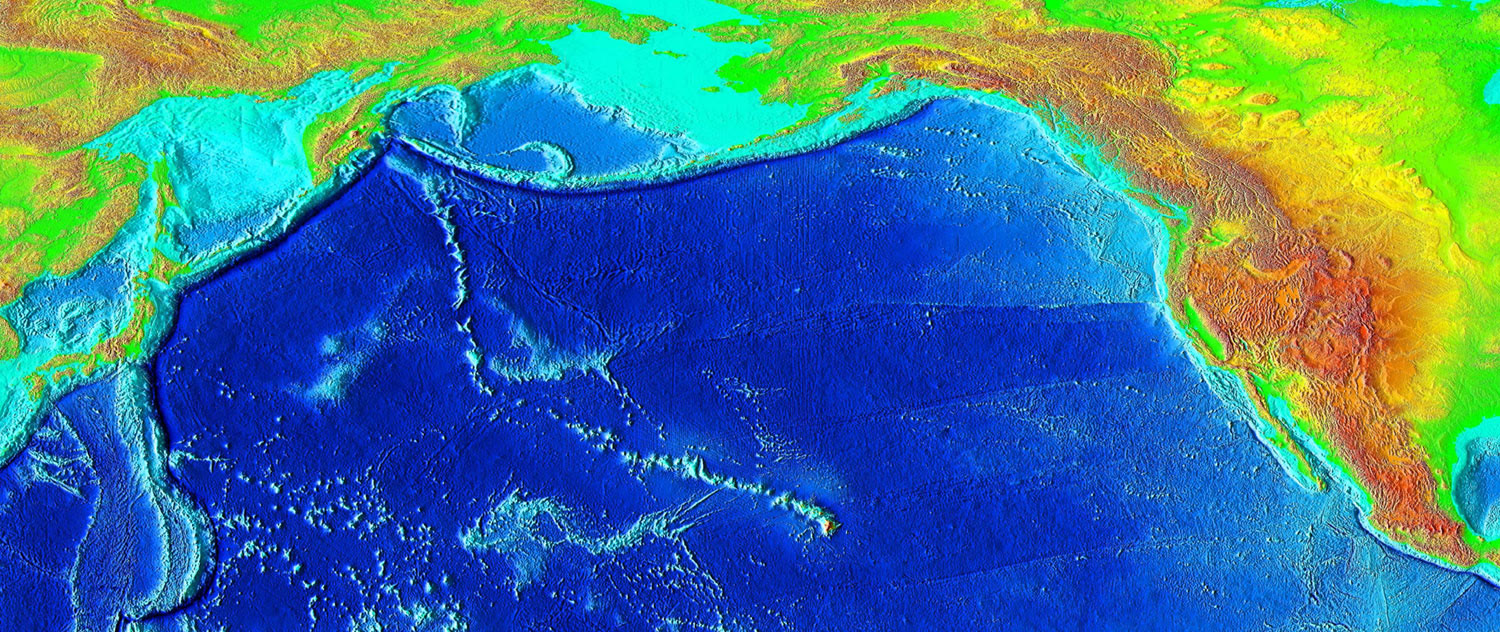
\includegraphics[width=\linewidth]{images/book2/g11-ngdc-hawaii-chain.jpg}

{\small تضاريس مظللة لقاع شمال المحيط الهادئ. تمتد سلسلة هاواي
من جزيرة هاواي (في أسفل الوسط، بالبني) نحو
الغرب الشمالي الغربي؛ وعند الانحناء تنعطف شمالًا لتصير الجبال البحرية الإمبراطورية، التي
تنتهي عند الخندق الممتد على طول كامتشاتكا وجزر الأليوتيان. الصورة: المركز الوطني
للبيانات الجيوفيزيائية، الإدارة الوطنية للمحيطات والغلاف الجوي (ملك عام).}
\end{omfigure}
% ledger: photo:g11-hawaii-chain

يعطي التأريخ بالبوتاسيوم--الأرغون للابات من 37 بركانًا من السلسلة، جُمعت من
الجزر، أو جُرفت من الجبال البحرية، أو استُخرجت بالحفر عبر رواسبها،
أعمارَها (المخطط أدناه). فعمر ماونا كيا نحو
\num{0.4} مليون سنة، وكاواي \num{5.1}، وميدواي \num{27.7}، وجبل
سويكو البحري، قرب الطرف البعيد لسلسلة الإمبراطور، \num{64.7}. وتزداد الأعمار
مع البعد عن كيلاويا، البركان النشط، كما يتنبأ \omterm{def:g11:plate-motions:hotspot-track}{أثر
البقعة الساخنة}.
% ledger: cd87:ages

\begin{omfigure}
\begin{tikzpicture}
\begin{axis}[ompt, width=0.82\linewidth, height=6.4cm, xmin=0, xmax=5000, ymin=0, ymax=70,
  xlabel={\foreignlanguage{arabic}{البعد عن كيلاويا على امتداد السلسلة \babelsublr{(\unit{km})}}}, ylabel={\foreignlanguage{arabic}{العمر بملايين السنين}},
  xticklabel style={/pgf/number format/set thousands separator={}},
  legend style={font=\scriptsize, at={(0.03,0.97)}, anchor=north west}, legend cell align=left]
% computed in figdata/grade-11/hawaii_chain.py; ledger: cd87:ages
\addplot[only marks, mark=o, mark size=1.6pt, omDef, error bars/.cd, y dir=both, y explicit]
  table[x=dist, y=age, y error=err] {figdata/out/grade-11-hawaii_chain-hawaiian.dat};
\addplot[only marks, mark=triangle, mark size=2pt, omProp, error bars/.cd, y dir=both, y explicit]
  table[x=dist, y=age, y error=err] {figdata/out/grade-11-hawaii_chain-emperor.dat};
\addplot[black, densely dashed, line width=0.6pt] table[x=dist, y=age] {figdata/out/grade-11-hawaii_chain-fit.dat};
\legend{{سلسلة هاواي}, {الانحناء وسلسلة الإمبراطور}, {\foreignlanguage{arabic}{مستقيم مار بالأصل، \babelsublr{\qty{9.1}{cm}} في السنة}}}
\draw[black!50, densely dotted] (axis cs:3400,0) -- (axis cs:3400,70);
\node[font=\scriptsize, anchor=south, rotate=90] at (axis cs:3400,8) {الانحناء};
\node[font=\scriptsize, anchor=north west] at (axis cs:519,5.1) {كاواي};
\node[font=\scriptsize, anchor=south] at (axis cs:2432,30) {ميدواي};
\node[font=\scriptsize, anchor=south east] at (axis cs:4860,65.5) {سويكو};
\end{axis}
\end{tikzpicture}

{\small عمر براكين سلسلة هاواي--الإمبراطور بدلالة
بعدها عن كيلاويا، مع أوجه عدم اليقين في الأعمار. فعلى امتداد
سلسلة هاواي تتبع النقاط مستقيمًا يمر بالأصل؛ أما بعد
الانحناء فتزداد الأعمار أسرع مع المسافة. البيانات: كلاغ ودالريمبل
(1987).}
\end{omfigure}

على امتداد سلسلة هاواي، حتى نحو \qty{3300}{km}، تتبعثر النقاط
حول مستقيم يمر بالأصل. والمستقيم الذي يلائم على أفضل وجه البراكين الستة والعشرين
المؤرخة في هذا الجزء يرتفع مليون سنة كل
\qty{91}{km}: وبحسب \cref{prop:g11:plate-motions:hotspot}، تكون الصفيحة الهادئية قد
تحركت فوق البقعة الساخنة بنحو \qty{91}{km} في كل مليون سنة، أي \qty{9.1}{cm}
في السنة. ووجد واضعا الأعمار، بملاءمة السلسلة كلها على طريقتهما،
\qty{8.6}{cm} في السنة.
% ledger: cd87:ages (fit computed in hawaii_chain.py), cd87:rate

بعد الانحناء تزداد الأعمار أسرع مع المسافة: فعلى امتداد سلسلة
الإمبراطور تحركت الصفيحة أبطأ، بنحو \qty{6.5}{cm} في السنة في المتوسط
(أفضل مستقيم عبر الجبال البحرية التسعة المؤرخة). ثم إن السلسلة تغيّر
اتجاهها. فإذا كانت البقعة الساخنة قد بقيت في مكانها، فإن الانحناء يسجل تغيرًا في
اتجاه حركة الصفيحة الهادئية. وتضع أعمار أحدث
بداية الانحناء قرب جبل كيمي البحري، قبل نحو 50 مليون
سنة، في الوقت نفسه الذي أُعيد فيه تنظيم الظهرات المتوسعة في
المحيط الهادئ وظهرت أولى براكين الأقواس الجزرية على امتداد حافته الغربية:
لقد غيّرت الصفيحة مسارها.
% ledger: cd87:ages (Emperor fit computed in hawaii_chain.py), sc06:bend

\section{القدرة التنبؤية للنموذج}\label{sec:g11:plate-motions:predictive}

يقول نموذج الصفائح إن بضع صفائح صلبة تدور حول أقطاب دورانها،
وإن كل شيء تقريبًا يحدث عند حدودها. وقوته أن
القياسات التي تُجرى بطرق مختلفة تمامًا، وعلى فترات زمنية مختلفة جدًا،
تعطي الأجوبة نفسها.

\begin{itemize}
  \item \emph{الزلازل والبراكين} تتجمع على امتداد الحدود، ونوع
        الحد يتنبأ بنوعها: زلازل ضحلة على امتداد
        الظهرات، وزلازل عميقة قرب الخنادق وحدها (\cref{ch:g11:subduction-zones}).
  \item \emph{قاع المحيط} أحدث ما يكون على امتداد الظهرات، ويزداد قِدمًا
        بالابتعاد عنها، تماثليًا على الجانبين
        (\cref{ch:g11:drift-to-spreading}).
  \item \emph{الأحزمة الجبلية} ترتفع حيث تتقارب الصفائح: فالهند لا تزال تتحرك
        نحو أوراسيا بنحو \qty{4.5}{cm} في السنة عبر الهيمالايا،
        كما يُحسب من أقطاب الدوران (\cref{ch:g12:mountain-building}).
  \item \emph{السرعات تتفق بين الطرق}: يقارن الجدول أدناه
        السرعات المقيسة اليوم بتحديد المواقع بالأقمار الصناعية بتلك التي تتنبأ
        بها أقطاب الدوران، التي تأتي معدلات توسعها أساسًا من
        الشرائط المغناطيسية وتمثل متوسط الحركة على آخر
        \num{0.8} إلى \num{3.2} مليون سنة، وبالسرعة التي يسجلها
        أثر بقعة ساخنة على عشرات ملايين السنين.
\end{itemize}
% ledger: nnr56:poles, nnr56:data (India-Eurasia computed in plate_velocities.py at 85 E 28 N)

\begin{center}
\small
\begin{tabular}{|l|c|c|}
\hline
ما يقاس & الطريقة & السرعة (\unit{cm} في السنة) \\ \hline
ماونا كيا، الصفيحة الهادئية & تحديد المواقع بالأقمار الصناعية، 30 سنة & 7.2 \\
ماونا كيا، الصفيحة الهادئية & قطب الدوران & 6.9 \\
فيتسل، الصفيحة الأوراسية & تحديد المواقع بالأقمار الصناعية، 31 سنة & 2.6 \\
فيتسل، الصفيحة الأوراسية & قطب الدوران & 2.3 \\
الصفيحة الهادئية فوق بقعة هاواي الساخنة & أعمار البراكين، 40 مليون سنة & 9.1 \\ \hline
\end{tabular}
\end{center}
% ledger: data:b2-ngl-gnss, nnr56:poles, cd87:ages (all computed in figdata/grade-11)

تتفق سرعات أقطاب الدوران وسرعات المحطات في حدود
\qty{0.3}{cm} في السنة، مع أن الأولى متوسطات على ملايين السنين
والثانية على عقود فقط: فالصفائح تتحرك اليوم كما تحركت منذ ملايين
السنين. أما سرعة البقعة الساخنة فأكبر: فهي تقاس في إطار آخر، هو إطار
البقعة الساخنة نفسها، وعلى زمن أطول بكثير.

ويظهر نمط آخر حين تُقارن سرعات الصفائح الكاملة. فالصفائح
الأسرع، كوكوس ونازكا والهادئية والأسترالية وصفيحة بحر
الفلبين، لكل منها حافة طويلة تغوص في الوشاح عند خندق؛ ومتوسط
سرعاتها نحو \qty{6.5}{cm} في السنة. أما الصفائح التي ليست لها
حافة كهذه، ومنها الأوراسية وأمريكا الشمالية وأمريكا الجنوبية والإفريقية
والقطبية الجنوبية، فتتحرك بنحو \qty{2.4}{cm} في السنة في المتوسط. وهذا المفتاح لفهم
ما يحرك الصفائح يُتناول في \cref{ch:g11:subduction-zones}.
% ledger: nnr56:rms (means computed in plate_velocities.py)

\section{تمارين}

\begin{exercise}[$\star$]\label{exo:g11:plate-motions:1}
عرّف \omterm{def:g11:plate-motions:rigid-plate}{الصفيحة الصلبة}. أين يتجمع تشوه \omterm{def:g11:lithosphere-asthenosphere:lithosphere}{الغلاف الصخري}،
وأي رصد زلزالي يومي يبيّن ذلك؟
\end{exercise}

\begin{exercise}[$\star$]\label{exo:g11:plate-motions:2}
تتحرك محطة ماونا كيا \qty{72}{mm} في السنة. عبّر عن هذه السرعة
بالكيلومترات في كل مليون سنة. كم تتحرك المحطة في 30 سنة؟ وفي
مليون سنة؟
\end{exercise}

\begin{exercise}[$\star$]\label{exo:g11:plate-motions:3}
في عشر سنوات تحركت محطة \qty{30}{cm} نحو الشرق و\qty{40}{cm} نحو الشمال. جد
سرعتيها نحو الشرق ونحو الشمال، وسرعتها، والزاوية التي يصنعها اتجاهها مع
الشمال.
\end{exercise}

\begin{exercise}[$\star$]\label{exo:g11:plate-motions:4}
عرّف \omterm{def:g11:plate-motions:hotspot-track}{أثر البقعة الساخنة}. أين يقع أحدث بركان على امتداد سلسلة هاواي،
وفي أي اتجاه تزداد الأعمار؟ وماذا يخبرنا ذلك
عن الاتجاه الذي تتحرك فيه الصفيحة الهادئية؟
\end{exercise}

\begin{exercise}[$\star$]\label{exo:g11:plate-motions:5}
تقع كاواي على بعد \qty{519}{km} من كيلاويا على امتداد السلسلة، وأقدم لاباتها
عمرها \num{5.1} مليون سنة. بافتراض أن البقعة الساخنة ثابتة، بأي
سرعة متوسطة حملتها الصفيحة، بالكيلومترات في كل مليون سنة
وبالسنتيمترات في السنة؟
\end{exercise}

\begin{exercise}[$\star\star$]\label{exo:g11:plate-motions:6}
في مخطط سلسلتي المحطتين، تحركت محطة فيتسل نحو
\qty{63}{cm} نحو الشرق و\qty{48}{cm} نحو الشمال في 31 سنة. جد سرعتيها نحو الشرق ونحو الشمال،
وسرعتها، واتجاهها. وقارن سرعتها بسرعة محطة ماونا
كيا.
\end{exercise}

\begin{exercise}[$\star\star$]\label{exo:g11:plate-motions:7}
في آيسلندا، عند \ang{64.5} شمالًا و\ang{18} غربًا، تعطي أقطاب الدوران
صفيحةَ أمريكا الشمالية السرعة $(-10.5, +20.6)$ والصفيحةَ الأوراسية
السرعة $(+7.7, +16.3)$، بالملليمترات في السنة (الشرق، الشمال). (1) جد
سرعة أمريكا الشمالية بالنسبة إلى أوراسيا، ومقدارها واتجاهها.
(2) ماذا تمثل هذه السرعة للظهرة التي تعبر آيسلندا؟ (3) قارن
بالمعدل \qty{2}{cm} في السنة الذي يُذكر غالبًا لشمال الأطلسي.
\end{exercise}

\begin{exercise}[$\star\star$]\label{exo:g11:plate-motions:8}
تدور الصفيحة الهادئية بمقدار \ang{0.651} في كل مليون سنة. (1) جد سرعة
نقطة على بعد \ang{90} من قطب دورانها، بالسنتيمترات في السنة. (2) وسرعة
نقطة على بعد \ang{30} من القطب؟ (3) أين تنعدم السرعة على الصفيحة؟ وهل يمكن
أن تُعطى سرعة صفيحة كاملة برقم واحد؟
\end{exercise}

\begin{exercise}[$\star\star$]\label{exo:g11:plate-motions:9}
شمال الهيمالايا، عند \ang{28} شمالًا و\ang{85} شرقًا، تعطي أقطاب الدوران
الصفيحةَ الهندية السرعة $(+40.6, +38.6)$ والصفيحةَ الأوراسية
السرعة $(+24.0, -3.3)$، بالملليمترات في السنة (الشرق، الشمال). (1) جد سرعة
الهند بالنسبة إلى أوراسيا، ومقدارها واتجاهها. (2) لو بقيت
كما هي، فبكم تتقارب الصفيحتان في 10 ملايين سنة؟
\end{exercise}

\begin{exercise}[$\star\star$]\label{exo:g11:plate-motions:10}
يقع نيكر على بعد \qty{1058}{km} من كيلاويا وعمره \num{10.3} مليون سنة؛
ويقع ميدواي على بعد \qty{2432}{km} وعمره \num{27.7} مليون سنة. جد
سرعة الصفيحة فوق البقعة الساخنة بين زمني بناء البركانين.
وقارنها بالسرعة \qty{9.1}{cm} في السنة.
\end{exercise}

\begin{exercise}[$\star\star$]\label{exo:g11:plate-motions:11}
عند نقطة ما، تتحرك الصفيحة $A$ بسرعة \qty{3}{cm} في السنة نحو الشرق بالنسبة إلى الصفيحة $B$،
وتتحرك الصفيحة $B$ بسرعة \qty{4}{cm} في السنة نحو الشمال بالنسبة إلى الصفيحة $C$.
(1) ارسم مثلث السرعات وجد سرعة $A$ بالنسبة إلى $C$:
مقدارها واتجاهها. (2) ما سرعة $C$ بالنسبة إلى $A$؟
\end{exercise}

\begin{exercise}[$\star\star\star$]\label{exo:g11:plate-motions:12}
يقع ماونا كيا على بعد \qty{54}{km} من كيلاويا وعمره \num{0.375} مليون
سنة. (1) أي سرعة يعطيها للصفيحة؟ (2) يبلغ عرض البركان بضع عشرات من
الكيلومترات، وهو ينمو طوال عدة مئات من آلاف السنين. لنفترض أن
بعده عن البقعة الساخنة غير يقيني بمقدار \qty{25}{km}: فبين أي
قيمتين تقع السرعة عندئذ؟ (3) فسّر لماذا تعطي البراكين الفتية القريبة من
البقعة الساخنة تقديرًا رديئًا للسرعة، ولماذا تكون البراكين البعيدة عنها
أفضل.
\end{exercise}

\begin{exercise}[$\star\star\star$]\label{exo:g11:plate-motions:13}
تتبعثر المواقع الشهرية لمحطة بنحو \qty{5}{mm} حول
مستقيمها. وتُرى الحركة بوضوح متى تجاوزت عشرة أضعاف التبعثر.
(1) كم من الزمن يجب القياس لرؤية حركة محطة ماونا كيا بوضوح،
\qty{72}{mm} في السنة؟ (2) وحركة قدرها \qty{5}{mm} في السنة، كما
عبر منطقة تتشوه ببطء داخل قارة؟ (3) لماذا قيست سرعات
الصفائح من الشرائط المغناطيسية قبل أن تستطيع الأقمار الصناعية قياسها
بزمن طويل؟
\end{exercise}

\begin{exercise}[$\star\star\star$]\label{exo:g11:plate-motions:14}
على ظهرة وسط الأطلسي عند \ang{30} جنوبًا (\ang{13.5} غربًا)، تعطي أقطاب
الدوران صفيحةَ أمريكا الجنوبية السرعة $(-4.9, +11.0)$ والصفيحةَ
الإفريقية السرعة $(+27.1, +17.9)$، بالملليمترات في السنة (الشرق، الشمال).
(1) جد سرعة أمريكا الجنوبية بالنسبة إلى إفريقيا، ومقدارها
واتجاهها. (2) استنتج \omterm{def:g11:drift-to-spreading:spreading-rate}{معدل التوسع الكلي} ونصف \omterm{def:g11:drift-to-spreading:spreading-rate}{معدل التوسع} للظهرة.
(3) أعطت رواسب جنوب الأطلسي نصف معدل يقارب \qty{1.9}{cm}
في السنة متوسطًا على آخر 66 مليون سنة
(\cref{ch:g11:drift-to-spreading}). قارن، واقترح ما قد يعنيه
الفرق.
\end{exercise}

\begin{exercise}[$\star\star\star$]\label{exo:g11:plate-motions:15}
تتحرك محطة باطراد \qty{20}{mm} في السنة نحو الشرق. وفي منتصف
عشر سنوات من القياس تمامًا، يزيحها زلزال فجأة \qty{50}{mm}
نحو الغرب. (1) ارسم مخططًا لموقعها نحو الشرق بدلالة الزمن. (2) ما السرعة
التي يجدها المرء من الموقعين الأول والأخير وحدهما؟ (3) ما السرعة التي
يعطيها كل من نصفي السلسلة على حدة؟ (4) كيف ينبغي
للجيوديسي أن يتعامل مع قفزة كهذه؟
\end{exercise}

\section{مسألة: قراءة سلسلة هاواي--الإمبراطور}

\begin{problem}[{مسألة نهاية الأسبوع --- سرعة صفيحة مكتوبة بالبراكين}]
\label{pb:g11:plate-motions:1}
% values from Clague and Dalrymple 1987, Table 1.4 (ledger cd87:ages); fits computed in
% figdata/grade-11/hawaii_chain.py (v_hawaiian 91.2, v_emperor_free 64.6); bend sc06:bend;
% MKEA rates data:b2-ngl-gnss
يعطي الجدول البعد عن كيلاويا، مقيسًا على امتداد السلسلة،
وعمر ثلاثة عشر بركانًا من سلسلة هاواي--الإمبراطور بطريقة البوتاسيوم--الأرغون.
وكيلاويا هو البركان النشط فوق البقعة الساخنة؛ ويقع الانحناء بين أبوت
ودايكاكوجي.

\begin{center}
\small
\begin{tabular}{|l|c|c||l|c|c|}
\hline
البركان & البعد (\unit{km}) & العمر (\unit{Ma}) & البركان & البعد (\unit{km}) & العمر (\unit{Ma}) \\ \hline
ماونا كيا & 54 & 0.375 & أبوت & 3280 & 38.7 \\ \hline
كاواي & 519 & 5.1 & دايكاكوجي & 3493 & 42.4 \\ \hline
نيهوا & 780 & 7.2 & كوكو (الجنوبي) & 3758 & 48.1 \\ \hline
نيكر & 1058 & 10.3 & أوجين & 4102 & 55.2 \\ \hline
لايسان & 1818 & 19.9 & نينتوكو & 4452 & 56.2 \\ \hline
ميدواي & 2432 & 27.7 & سويكو (الوسط) & 4860 & 64.7 \\ \hline
كولاهان & 3128 & 38.6 & & & \\ \hline
\end{tabular}
\end{center}

\medskip
\noindent\textbf{الجزء الأول --- الأعمار والمسافات.}
\begin{enumerate}
  \item أي براكين الجدول أحدث، وأيها أقدم؟ وكيف
        تتغير الأعمار على امتداد السلسلة؟
  \item بيّن أن المسافة بالكيلومترات مقسومة على العمر بملايين
        السنين سرعة بالملليمترات في السنة.
  \item احسب السرعة المتوسطة $d/t$ التي تعطيها كاواي.
  \item احسب $d/t$ لنيكر ولايسان وميدواي وكولاهان وأبوت.
  \item ارسم العمر بدلالة المسافة للبراكين الثمانية في
        الجدول الواقعة قبل الانحناء. هل تقع النقاط قرب مستقيم يمر
        بالأصل؟
\end{enumerate}

\medskip
\noindent\textbf{الجزء الثاني --- سرعة الصفيحة فوق البقعة الساخنة.}
\begin{enumerate}[resume]
  \item فسّر لماذا، في حالة بقعة ساخنة ثابتة وصفيحة تتحرك بسرعة ثابتة
        $v$، يحقق العمر $t$ والمسافة $d$ العلاقة $t = d/v$.
  \item احسب متوسط السرعات الخمس في السؤال~4.
  \item المستقيم المار بالأصل الذي يلائم على أفضل وجه البراكين الستة والعشرين
        المؤرخة كلها في سلسلة هاواي يعطي \qty{91}{km} في كل مليون سنة.
        قارن بالسؤال~7.
  \item بهذه السرعة، كم من الزمن تحتاج الصفيحة لتحمل كاواي من
        البقعة الساخنة إلى موضعها الحالي؟ قارن بعمرها.
  \item في أي اتجاه تتحرك الصفيحة الهادئية فوق البقعة الساخنة؟
\end{enumerate}

\medskip
\noindent\textbf{الجزء الثالث --- الانحناء.}
\begin{enumerate}[resume]
  \item احسب السرعة المتوسطة للصفيحة بين زمني بناء دايكاكوجي
        وسويكو (الوسط).
  \item أفضل مستقيم عبر البراكين التسعة المؤرخة ابتداءً من
        دايكاكوجي يعطي \qty{65}{km} في كل مليون سنة. قارن
        بالسرعة على امتداد سلسلة هاواي.
  \item تضع أعمار أحدث بداية الانحناء قرب جبل كيمي
        البحري، على بعد \qty{3668}{km} من كيلاويا، قبل نحو 50 مليون سنة.
        فأي سرعة متوسطة يعطيها ذلك لسلسلة هاواي كلها؟
        قارن بالسرعة \qty{91}{km} في كل مليون سنة، وفسّر لماذا يمكن أن تكون
        القيمتان كلتاهما صحيحتين.
  \item إذا كانت البقعة الساخنة قد بقيت ثابتة، فماذا يسجل الانحناء عن
        الصفيحة الهادئية؟
  \item وجد التأريخ الأحدث تغيرات كبيرة في السرعة على امتداد سلسلة الإمبراطور
        مع تغير ضئيل في اتجاهها. فسّر لماذا يكون اتجاه
        السلسلة وتباعد أعمارها معلومتين مستقلتين.
\end{enumerate}

\medskip
\noindent\textbf{الجزء الرابع --- المقارنة بقياس الأقمار الصناعية اليوم.}
\begin{enumerate}[resume]
  \item تتحرك محطة ماونا كيا بسرعة $\qty{-63.2}{mm}$ في السنة نحو الشرق
        و$\qty{+34.5}{mm}$ في السنة نحو الشمال. جد مقدار سرعتها واتجاهها.
  \item تمتد سلسلة هاواي من كيلاويا نحو الغرب الشمالي الغربي. فهل
        يتسق اتجاه المحطة معها؟
  \item تعطي المحطة \qty{7.2}{cm} في السنة، والسلسلة \qty{9.1}{cm} في السنة.
        أعط سببين لعدم وجوب تساوي الرقمين.
  \item بسرعة \qty{91}{km} في كل مليون سنة، كم من الزمن ستحتاج الصفيحة
        لتحمل ماونا كيا مسافة \qty{100}{km} أخرى بعيدًا عن البقعة الساخنة؟
  \item استنتج: بأي سرعة تحركت الصفيحة الهادئية فوق بقعة هاواي
        الساخنة خلال آخر 40 مليون سنة؟
\end{enumerate}
\end{problem}
